\documentclass[tikz,border=8pt]{standalone}
\usepackage{tikz}
\usetikzlibrary{arrows.meta,decorations.pathreplacing,calc,patterns}

% Brand palette
\definecolor{garnet}{HTML}{73000A}
\definecolor{atlantic}{HTML}{466A9F}
\definecolor{horseshoe}{HTML}{65780B}
\definecolor{ink}{HTML}{363636}
\definecolor{warmgrey}{HTML}{676156}

\begin{document}
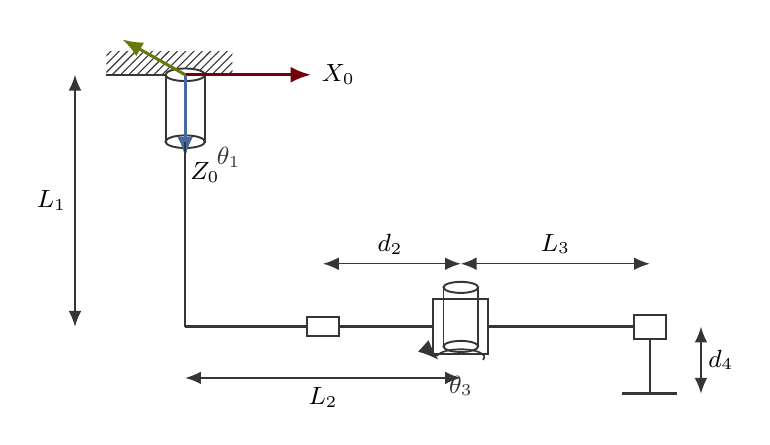
\begin{tikzpicture}[
    >={Latex[length=2.6mm,width=2mm]},
    line cap=butt, line join=miter,
    every node/.style={font=\small},
    link/.style={ink, line width=0.9pt},
    axis/.style={line width=1.1pt},
    dim/.style={ink, line width=0.5pt, <->, >={Latex[length=2mm,width=1.6mm]}},
    joint/.style={ink, fill=white, line width=0.7pt},
]

% --- Ceiling (hatched) ---
\fill[pattern=north east lines, pattern color=ink]
    (-1.0,5.4) rectangle (0.6,5.7);
\draw[ink, line width=0.6pt] (-1.0,5.4) -- (0.6,5.4);

% --- Base (joint 1) cylinder mounted to ceiling ---
% Cylinder body
\draw[joint] (-0.25,4.55) rectangle (0.25,5.4);
\draw[joint] (0,5.4) ellipse (0.25 and 0.08);
\draw[joint] (0,4.55) ellipse (0.25 and 0.08);

% Frame {0} axes at top of cylinder
\draw[axis,garnet,->]   (0,5.4) -- ++(1.6,0) node[right,black] {$X_0$};
\draw[axis,atlantic,->] (0,5.4) -- ++(0,-1.05) node[below right=-2pt,black] {$Z_0$};
\draw[axis,horseshoe,->] (0,5.4) -- ++(-0.8,0.45) node[above left=-3pt,black] {};

% Theta_1 label near rotation axis
\node[ink] at (0.55,4.35) {$\theta_1$};

% --- Vertical link L1 ---
\draw[link] (0,4.55) -- (0,2.2);

% L1 dimension on the far left
\draw[dim] (-1.4,5.4) -- (-1.4,2.2);
\node at (-1.7,3.8) {$L_1$};

% --- Horizontal link L2 ---
\draw[link] (0,2.2) -- (3.5,2.2);

% Small fixed coupling box on L2 (matches sketch)
\draw[joint] (1.55,2.08) rectangle (1.95,2.32);

% L2 dimension below
\draw[dim] (0,1.55) -- (3.5,1.55);
\node at (1.75,1.3) {$L_2$};

% --- Joint 3: vertical revolute cylinder at x = 3.5 ---
% Outer mounting block
\draw[joint] (3.15,1.85) rectangle (3.85,2.55);
% Cylinder of joint 3
\draw[joint] (3.5,2.7) ellipse (0.22 and 0.07);
\draw[joint] (3.28,2.7) -- (3.28,1.95);
\draw[joint] (3.72,2.7) -- (3.72,1.95);
\draw[joint] (3.5,1.95) ellipse (0.22 and 0.07);
% Curved arrow indicating rotation
\draw[ink, line width=0.6pt, ->]
    (3.78,1.78) arc (-20:200:0.30 and 0.10);
\node[ink] at (3.5,1.45) {$\theta_3$};

% d2 dimension between joint axis (x=0) is wrong; in sketch d2 spans from L2 end region to joint 3.
% Per sketch d2 is between the small coupling box and joint 3
\draw[dim] (1.75,3.0) -- (3.5,3.0);
\node at (2.6,3.25) {$d_2$};

% --- Link L3 to the right of joint 3 ---
\draw[link] (3.85,2.2) -- (5.9,2.2);

% L3 dimension above
\draw[dim] (3.5,3.0) -- (5.9,3.0);
\node at (4.7,3.25) {$L_3$};

% --- End effector / prismatic d4 ---
% End block
\draw[joint] (5.7,2.05) rectangle (6.1,2.35);
% Prismatic shaft going down
\draw[link] (5.9,2.05) -- (5.9,1.35);
% End plate
\draw[link] (5.55,1.35) -- (6.25,1.35);

% d4 dimension on the right
\draw[dim] (6.55,2.2) -- (6.55,1.35);
\node at (6.8,1.78) {$d_4$};

\end{tikzpicture}
\end{document}
